\documentclass[acmsmall,nonacm]{acmart}
\makeatletter
\renewcommand\@formatdoi[1]{\ignorespaces}
\makeatother

\usepackage{subcaption}
\usepackage{float}
\usepackage{tabularx}
\usepackage{graphicx}
\usepackage{caption}


%%
%% \BibTeX command to typeset BibTeX logo in the docs
\AtBeginDocument{%
  \providecommand\BibTeX{{%
    \normalfont B\kern-0.5em{\scshape i\kern-0.25em b}\kern-0.8em\TeX}}}


\begin{document}

%\begin{titlepage}
%\end{titlepage}

%%
%% The "title" command has an optional parameter,
%% allowing the author to define a "short title" to be used in page headers.
\title{AI Dependability Assessment} % TODO find a good title

%%
%% The "author" command and its associated commands are used to define
%% the authors and their affiliations.
%% Of note is the shared affiliation of the first two authors, and the
%% "authornote" and "authornotemark" commands
%% used to denote shared contribution to the research.

\author{Patrick Deutschmann}
\email{patrick.deutschmann@student.tugraz.at}

\author{Lukas Timpl}
\email{lukas.timpl@student.tugraz.at}


%%
%% The abstract is a short summary of the work to be presented in the
%% article.
\begin{abstract}
% TODO write abstract
\end{abstract}

%%
%% The code below is generated by the tool at http://dl.acm.org/ccs.cfm.
%% Please copy and paste the code instead of the example below.
%%
%\begin{CCSXML}
%<ccs2012>
%   <concept>
%       <concept_id>10010147.10010178.10010179</concept_id>
%       <concept_desc>Computing methodologies~Natural language processing</concept_desc>
%       <concept_significance>500</concept_significance>
%       </concept>
% </ccs2012>
%\end{CCSXML}

%%
%% This command processes the author and affiliation and title
%% information and builds the first part of the formatted document.
\maketitle

\tableofcontents


\section{Introduction}

This is a submission to the \textit{Siemens AI Dependability Assessment}\footnote{\url{https://ecosystem.siemens.com/ai-da-sc}}. The challenge task was to solve a 2D binary classification problem, i.e. a binary function $f(\mathbf{x})$ classifies a data point $\mathbf{x_i} = (x_i^1, x_i^2)$ as either $l_i=0$ (green) or $l_i=1$ (red). With only two dimensions, the data sets are rather simple, yet the approach should also scale to inputs of higher dimensions. Most importantly, however, $f(\mathbf{x})$ should provide safety guarantees. This means that the ML model must not only have high predictive capabilities but also be capable of producing provably reliable results under certain assumptions. Furthermore, the setting is chosen such that misclassification costs are not equal for the two classes. Following the analogy of traffic lights, it is more dangerous (costly) to classify a red sample as green than classifying a green sample as red.  

Our solution aims at striking the ideal balance of these criteria in that it displays high predictive performance, gives provable safety guarantees, scales well to more complex data sets, and lets domain experts dynamically configure the class-wise cost of misclassification.

The architecture we chose is a deep neural network trained with cost-weighted binary cross-entropy loss. The safety guarantees follow the assumption of reliable training inputs. Using Linear Relaxation Based Perturbation Analysis (LiRPA), we can guarantee stable predictions in the epsilon neighbourhood of previously seen samples.

\subsection{Data sets}

Fig. \ref{fig:datasets} shows the three data sets of the challenge. Before we started our experiments, we analysed them and found that they differ in multiple critical aspects. 

\begin{enumerate}
	\item \textbf{Size}: The data sets vary in size, with A being the smallest and C the biggest.
	\item \textbf{Class balance}: While data set B is relatively balanced, A and C show significant imbalance with a ratio of roughly 2:1 and 10:1, respectively, where class 0 (green) is the overrepresented one.
	\item \textbf{Separability}: It is easy to see that data set B can be separated by drawing a simple sine-like wave across the two dimensions and data set B by using multiple ellipses. For data set A, however, it is harder to make out a clear trend. There are several cases where green and red samples are very close to each other, and accurately separating classes will prove difficult.
\end{enumerate}

Thus, while we employ the same general approach for all three data sets, we tune our hyper-parameters separately to obtain ideal performance. We use simpler models for smaller data sets to prevent overfitting and counter class imbalance by using a weighted loss, as detailed in Section \ref{sec:approach}. % TODO really true that we use simpler model for data set A?

\begin{figure}
\centering
\begin{subfigure}{.32\textwidth}
  \centering
  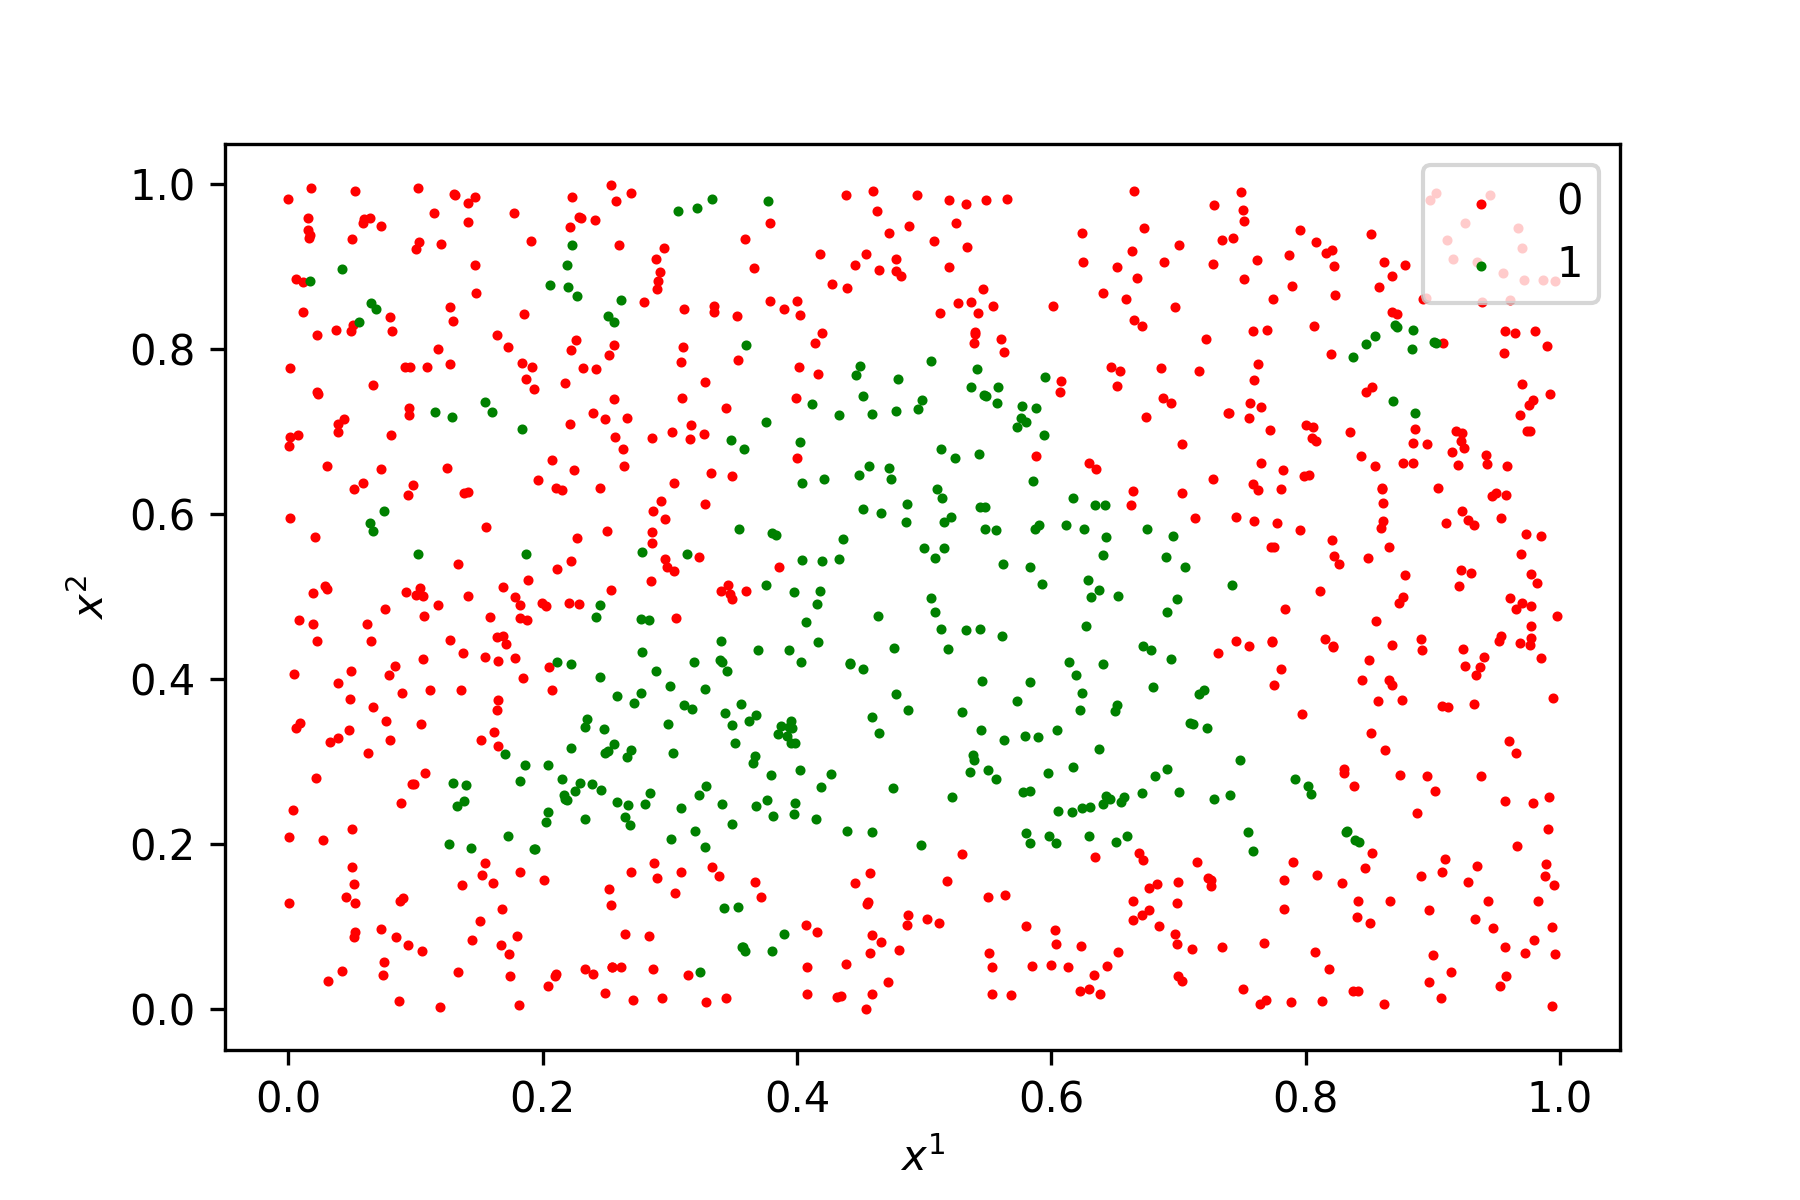
\includegraphics[width=\textwidth]{assets/ds_a.png}
  \caption{1,000 samples}
\end{subfigure}
\begin{subfigure}{.32\textwidth}
  \centering
  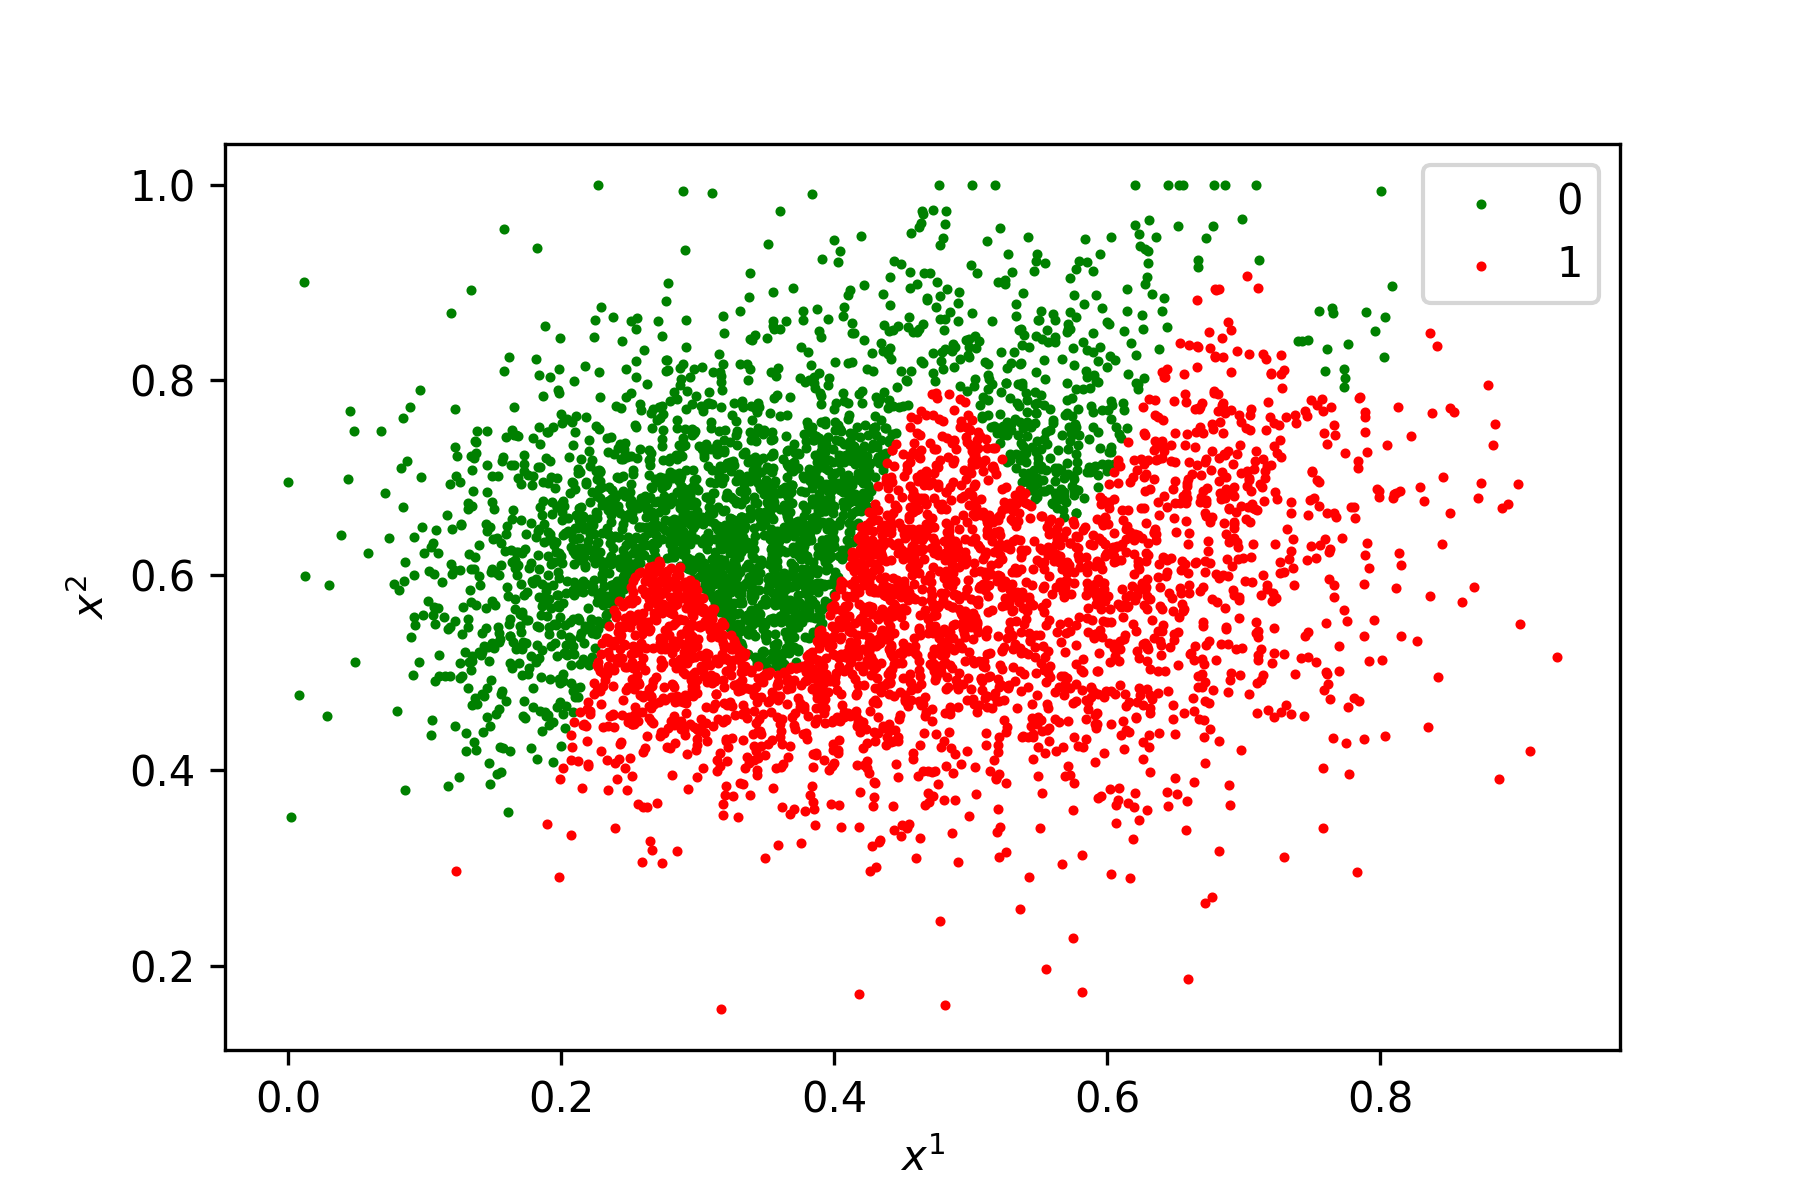
\includegraphics[width=\textwidth]{assets/ds_b.png}
  \caption{5,000 samples}
\end{subfigure}
\begin{subfigure}{.32\textwidth}
  \centering
  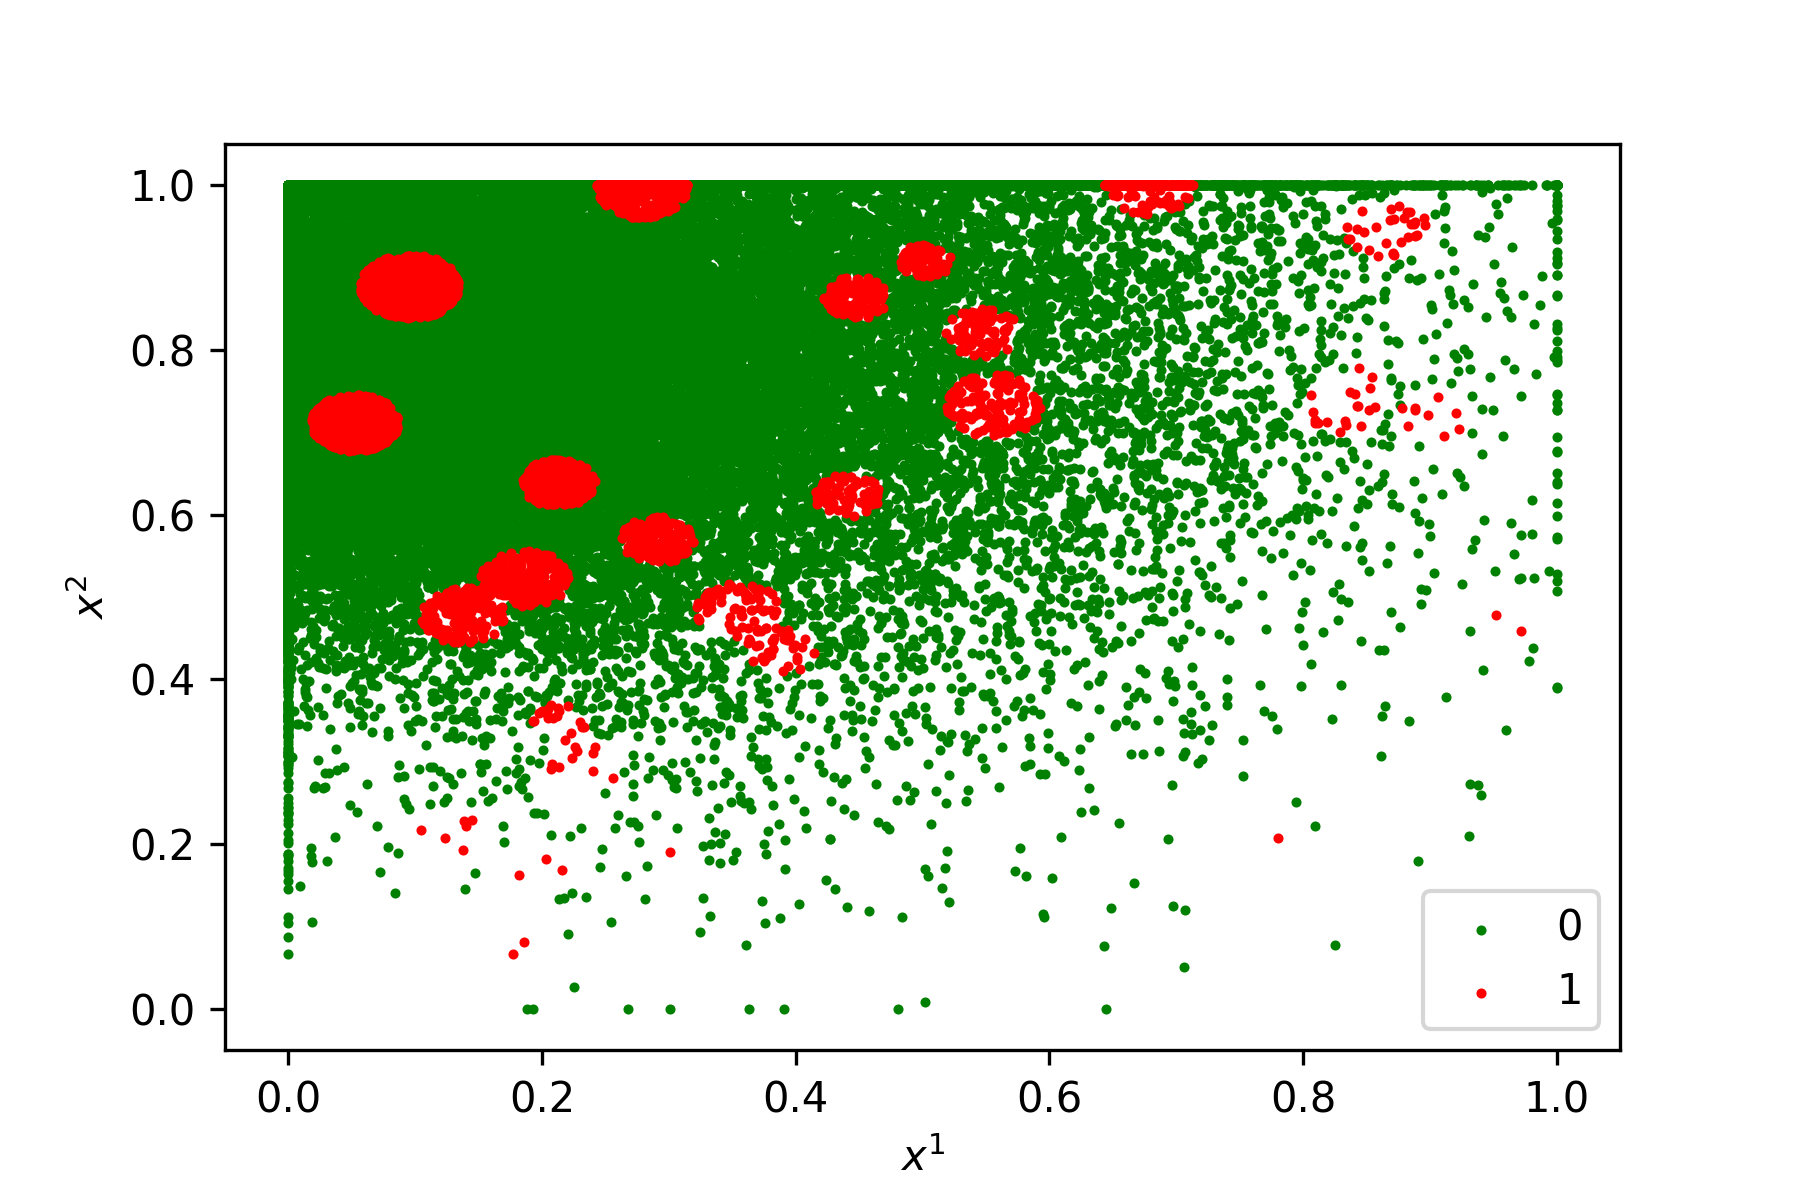
\includegraphics[width=\textwidth]{assets/ds_c.png}
  \caption{50,000 samples}
\end{subfigure}
\caption{The data sets of the challenge differ significantly in size, class balance and separability.}
\label{fig:datasets}
\end{figure}


\section{Possible Solutions and Related Work}
% - possible approaches + related work

\section{Approach} \label{sec:approach}
%TODO
%• A description of the employed ML approach
%• All assumptions made, including an exhaustive proposal/justification for their validation
~\cite{xu2020automatic}

\section{Results}
%TODO
% For each data set, an upper bound for the misclassification error, including its justification

We used Weights \& Biases \cite{wandb} for experiment tracking and visualisations.


\section{Scaling to higher dimensions}
%TODO
% An outline how the approach could be scaled to higher dimensions

\section{Appendix}
%TODO
% In an appendix, the documented code should be supplied

\pagebreak  

%%
%% The next two lines define the bibliography style to be used, and
%% the bibliography file.
\bibliographystyle{ACM-Reference-Format}

\bibliography{references}
% References to results that are used


\end{document}
\endinput

